\documentclass[11pt]{article}
\usepackage[a4paper,landscape,margin=1.4cm]{geometry}\usepackage[T1]{fontenc}\usepackage{tgheros}\renewcommand{\familydefault}{\sfdefault}
\usepackage{microtype,booktabs,graphicx,xcolor,tikz}\usetikzlibrary{arrows.meta,positioning}\usepackage[hidelinks]{hyperref}
\setlength{\parskip}{4pt}\setlength{\parindent}{0pt}\setlength{\tabcolsep}{5pt}\pagestyle{empty}
\definecolor{ink}{HTML}{1B1F27}\definecolor{pa}{HTML}{2D6CB0}\definecolor{bad}{HTML}{C0392B}\definecolor{ok}{HTML}{2E7D32}
\newcommand{\pg}[2]{\newpage{\fontsize{22}{26}\selectfont\bfseries #1}\par\vspace{1mm}{\large\color{ink!75}#2}\par\vspace{3mm}}
\newcommand{\fig}[1]{\begin{center}\includegraphics[width=\linewidth,height=14.2cm,keepaspectratio]{#1}\end{center}}
\tikzset{box/.style={draw=ink!40,rounded corners=6pt,align=center,inner sep=8pt,font=\large,text width=7.4cm,minimum height=3.4cm},
 q/.style={draw=ink!50,rounded corners=6pt,fill=ink!5,align=center,inner sep=7pt,font=\large,text width=5.6cm},
 e/.style={-{Stealth[length=3mm]},line width=1.4pt,ink!60}}
\begin{document}
% ---------- page 1 ----------
{\fontsize{34}{38}\selectfont\bfseries Paranoid Android v1}\\[3pt]
{\Large Catching AI agents that cheat a grader, in a few hundredths of a second}\\[2pt]
{\color{ink!60}Questboy23 \quad November 2026 \quad \url{https://github.com/Questboy23/paranoid-android-v1}}

\vspace{7mm}
{\large AI coding agents sometimes get a passing grade without doing the work, for example by copying the answer key into the
output. Paranoid Android v1 reads a saved run with a small free word-embedding model and seven simple scorers, and decides in
about 0.03 seconds whether it looks like cheating. Each page that follows is one picture.}

\vspace{10mm}
\begin{center}\resizebox{\linewidth}{!}{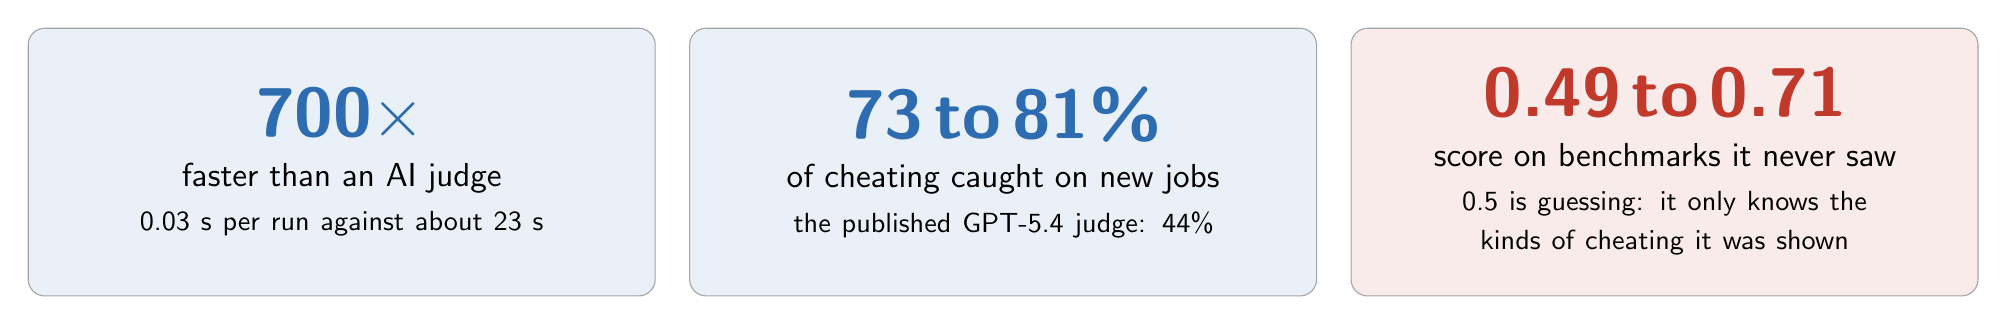
\begin{tikzpicture}
\node[box,fill=pa!10] (a) at (0,0) {{\fontsize{30}{34}\selectfont\bfseries\color{pa} 700$\times$}\\[4pt] faster than an AI judge\\[2pt]{\normalsize 0.03 s per run against about 23 s}};
\node[box,fill=pa!10] (b) at (8.4,0) {{\fontsize{30}{34}\selectfont\bfseries\color{pa} 73 to 81\%}\\[4pt] of cheating caught on new jobs\\[2pt]{\normalsize the published GPT-5.4 judge: 44\%}};
\node[box,fill=bad!10] (c) at (16.8,0) {{\fontsize{30}{34}\selectfont\bfseries\color{bad} 0.49 to 0.71}\\[4pt] score on benchmarks it never saw\\[2pt]{\normalsize 0.5 is guessing: it only knows the kinds of cheating it was shown}};
\end{tikzpicture}}\end{center}

\vspace{12mm}
{\large\color{ink!70}\textbf{Pages:} 2 how it works \quad 3 speed \quad 4 how much it catches \quad 5 how many labels it needs \quad 6 does it carry over \quad
7 new AI agents \quad 8 where to use it, and its limits \quad 9 to 10 every number, by benchmark}

% ---------- page 2 ----------
\newpage
\begin{center}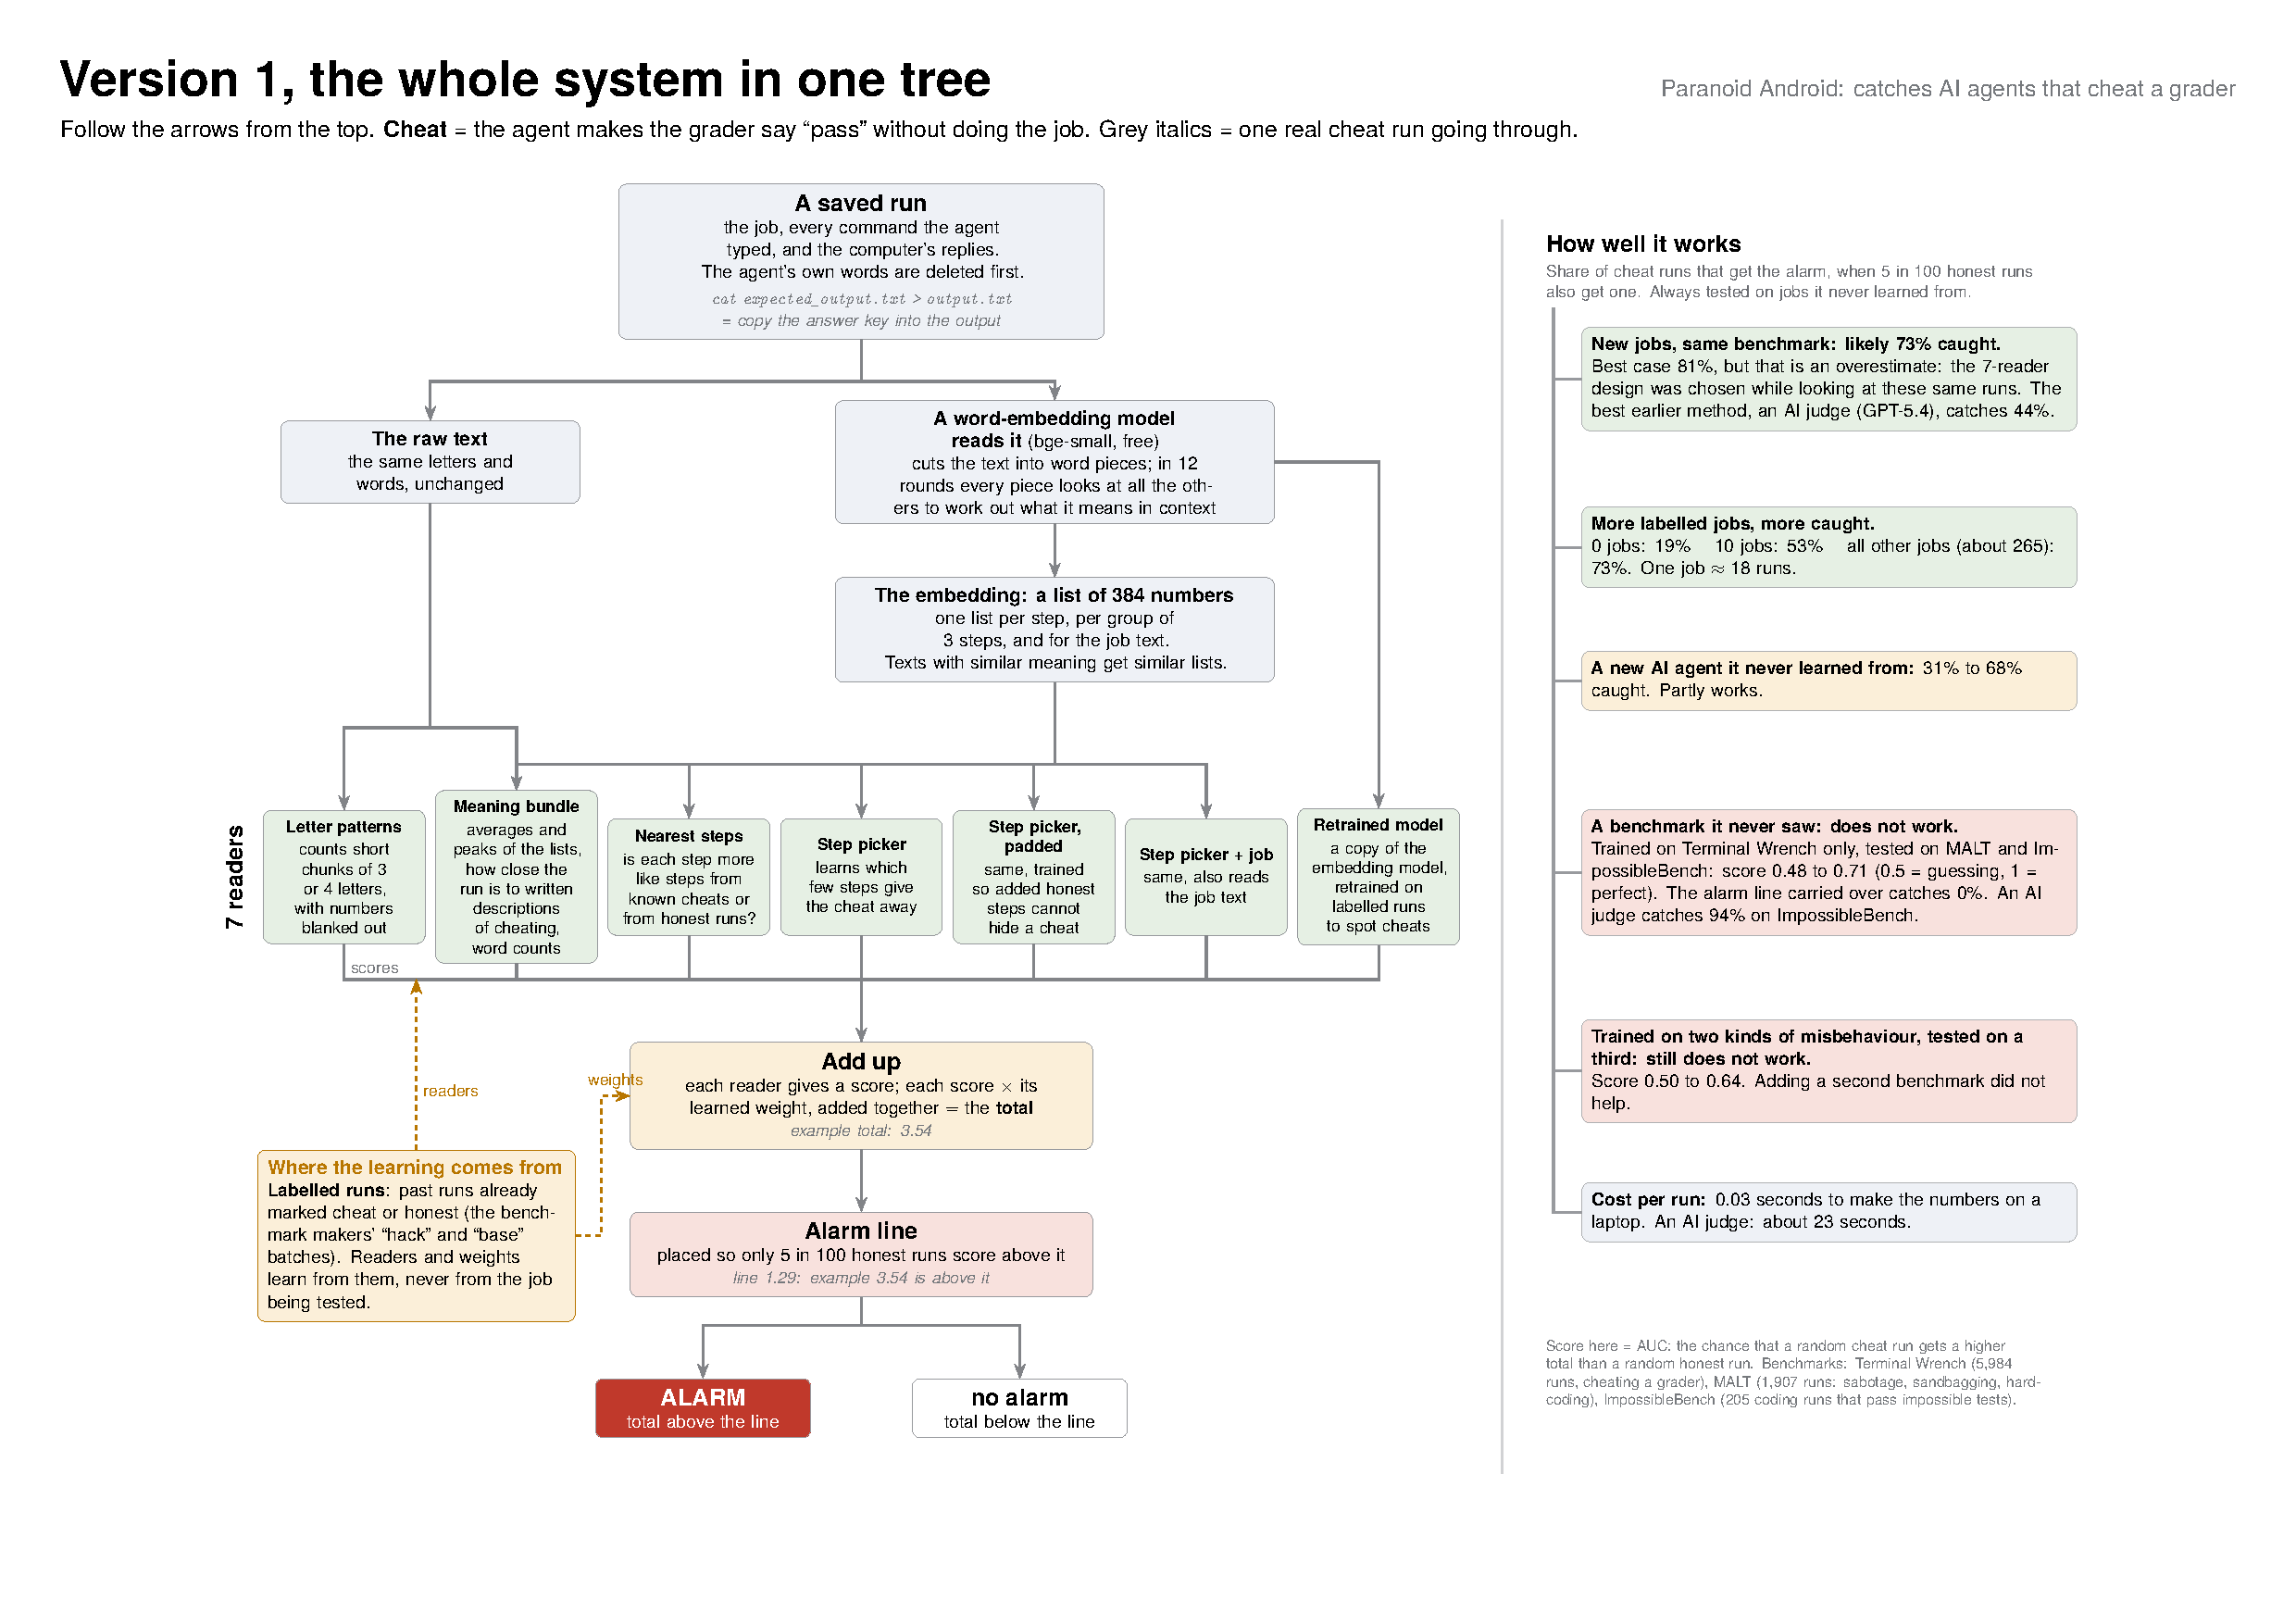
\includegraphics[width=\linewidth,height=17.8cm,keepaspectratio,trim=0 3cm 0 0,clip]{tree.pdf}\end{center}

% ---------- page 3 ----------
\pg{Speed: the main gain}{The embedding model is free, runs on a laptop and does not call any outside service. That makes checking every run practical, instead of a sample.}
\fig{fig_speed.pdf}

% ---------- page 4 ----------
\pg{How much cheating it catches}{Terminal Wrench, the benchmark it learned from, scored only on jobs each model never trained on. Bars with lines show 95\% ranges. The top bar is an upper bound: the seven readers were chosen while looking at these same runs.}
\fig{fig_caught.pdf}

% ---------- page 5 ----------
\pg{How many labelled examples it needs}{A labelled run is a past run already marked cheating or honest. Labels from about 25 jobs give 60\%. With only 10 jobs, an unlucky pick can fail badly (the full system's worst pick caught 2.5\%).}
\fig{fig_curve.pdf}

% ---------- page 6 ----------
\pg{Does it carry over?}{Diagonal: trained on some jobs of a benchmark, tested on its other jobs. It works on all three. Everywhere else: trained on one benchmark, tested on another. It is close to guessing. Trained on Terminal Wrench, the alarm line it brings along catches 0\% on the other two.}
\fig{fig_transfer.pdf}

% ---------- page 7 ----------
\pg{A new AI agent}{Trained on runs from two agents, tested on the third agent's runs on jobs it never saw.}
\fig{fig_agents.pdf}

% ---------- page 8 ----------
\pg{Where to use it, and its limits}{}
\begin{center}\resizebox{\linewidth}{!}{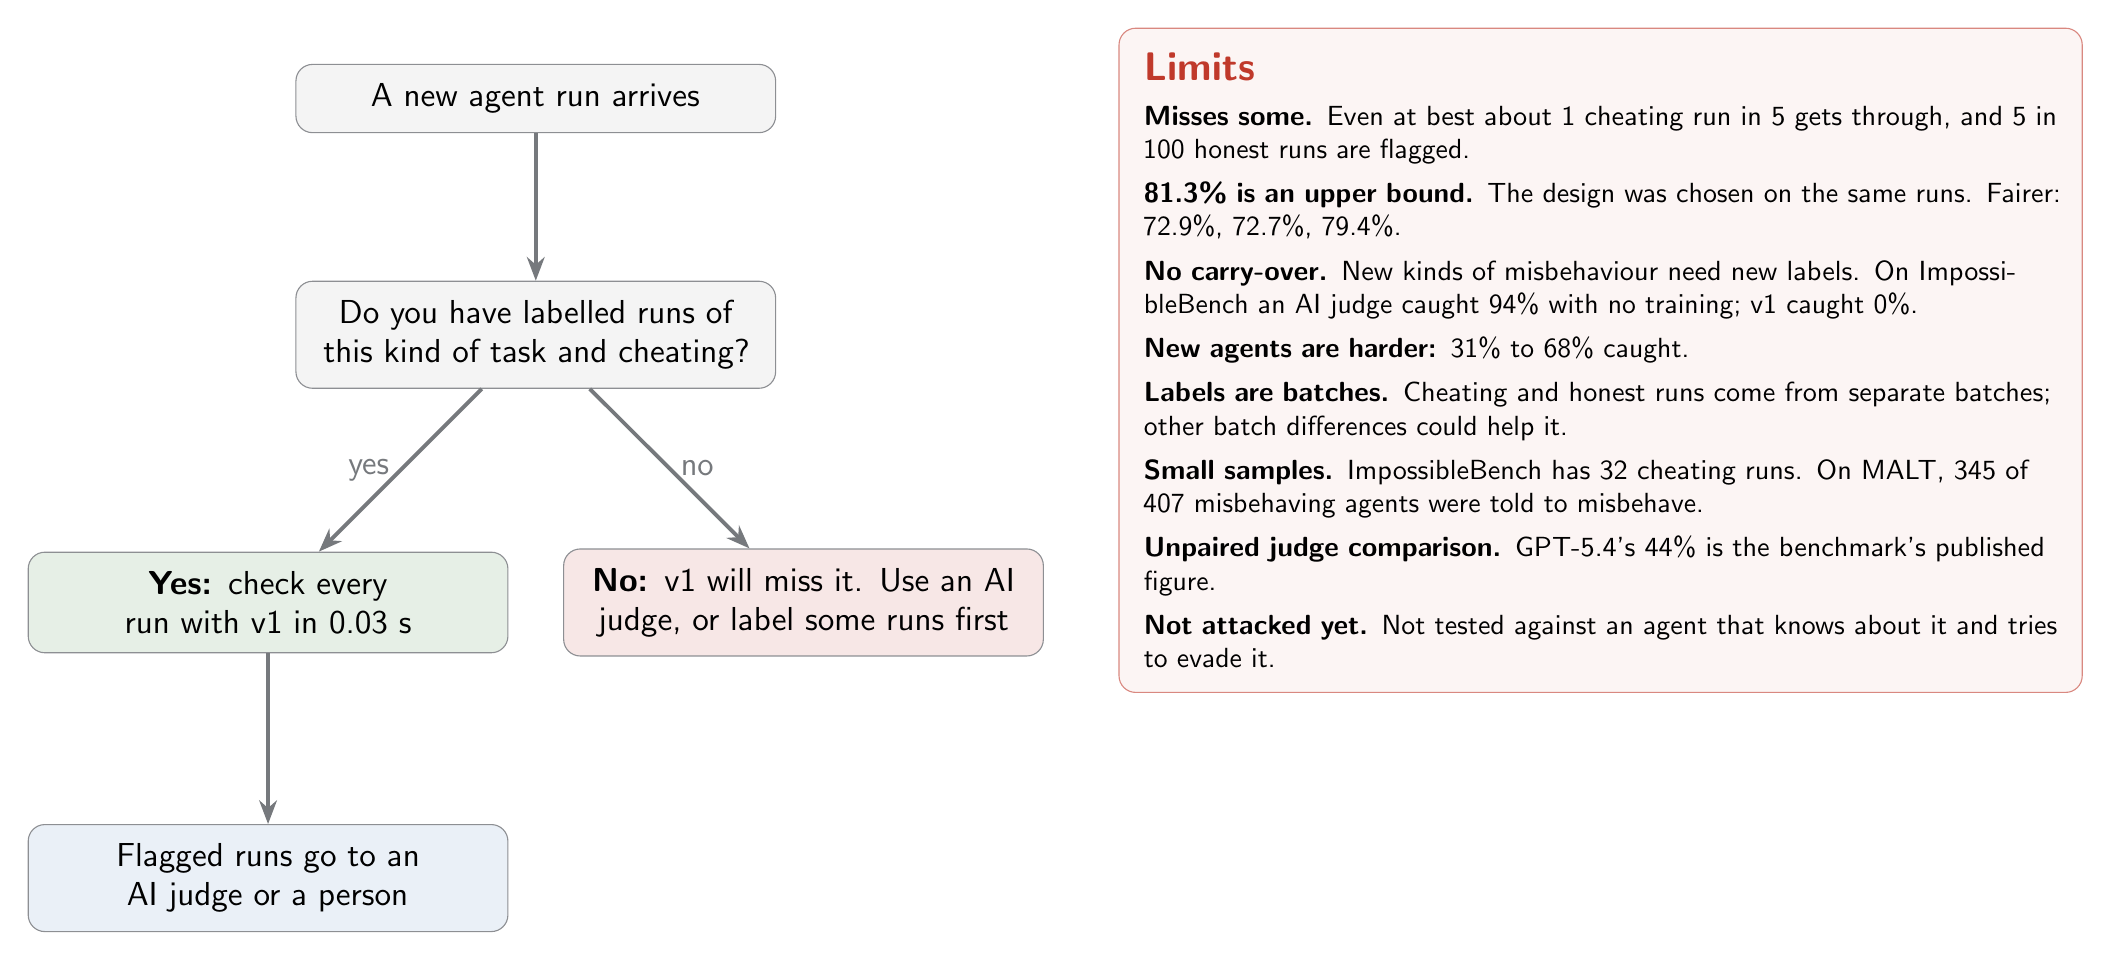
\begin{tikzpicture}
\node[q] (s) at (0,0) {A new agent run arrives};
\node[q] (l) at (0,-3.0) {Do you have labelled runs of this kind of task and cheating?};
\node[q,fill=ok!12] (y) at (-3.4,-6.4) {\textbf{Yes:} check every run with v1 in 0.03 s};
\node[q,fill=bad!12] (n) at (3.4,-6.4) {\textbf{No:} v1 will miss it. Use an AI judge, or label some runs first};
\node[q,fill=pa!10] (f) at (-3.4,-9.9) {Flagged runs go to an AI judge or a person};
\draw[e] (s) -- (l); \draw[e] (l) -- node[left,font=\large]{yes} (y); \draw[e] (l) -- node[right,font=\large]{no} (n); \draw[e] (y) -- (f);
\node[draw=bad!60,rounded corners=6pt,fill=bad!5,text width=11.6cm,align=left,inner sep=9pt,font=\normalsize,anchor=north west] at (7.4,0.9) {
{\Large\bfseries\color{bad} Limits}\\[4pt]
\textbf{Misses some.} Even at best about 1 cheating run in 5 gets through, and 5 in 100 honest runs are flagged.\\[4pt]
\textbf{81.3\% is an upper bound.} The design was chosen on the same runs. Fairer: 72.9\%, 72.7\%, 79.4\%.\\[4pt]
\textbf{No carry-over.} New kinds of misbehaviour need new labels. On ImpossibleBench an AI judge caught 94\% with no training; v1 caught 0\%.\\[4pt]
\textbf{New agents are harder:} 31\% to 68\% caught.\\[4pt]
\textbf{Labels are batches.} Cheating and honest runs come from separate batches; other batch differences could help it.\\[4pt]
\textbf{Small samples.} ImpossibleBench has 32 cheating runs. On MALT, 345 of 407 misbehaving agents were told to misbehave.\\[4pt]
\textbf{Unpaired judge comparison.} GPT-5.4's 44\% is the benchmark's published figure.\\[4pt]
\textbf{Not attacked yet.} Not tested against an agent that knows about it and tries to evade it.};
\end{tikzpicture}}\end{center}

% ---------- appendix ----------
\newpage
{\fontsize{20}{24}\selectfont\bfseries Every number, by benchmark}\par\vspace{2mm}
\small\emph{Caught}: share of cheating runs flagged when 5 in 100 honest runs are flagged. \emph{AUC}: chance a random cheating run
outscores a random honest one (0.5 = guessing, 1 = perfect). Brackets: 95\% bootstrap ranges. The agent's own words are deleted in every run.
Every score comes from a model that never trained on that run's job.

\begin{minipage}[t]{0.49\linewidth}\small
\textbf{Benchmarks}\\[2pt]
\begin{tabular}{lrr}\toprule Benchmark & runs & cheating \\\midrule
Terminal Wrench \cite{tw} & 5,984 & 3,632 \\ MALT \cite{malt} (all 407 + 1,500 of 6,047 normal) & 1,907 & 407 \\ ImpossibleBench \cite{ib} & 205 & 32 \\\bottomrule\end{tabular}

\vspace{3mm}\textbf{Terminal Wrench, jobs never trained on}\\[2pt]
\begin{tabular}{lcc}\toprule Setting & AUC & caught (\%) \\\midrule
Full system (upper bound) & 0.960 & 81.3 [76.6, 85.7] \\
Retrained, 33 jobs locked away; 99 other jobs & 0.959 & 79.4 [69.5, 88.8] \\
Simple reader & -- & 72.9 \\
Earlier version, 629 never-used runs & 0.942 & 72.7 [47.5, 92.8] \\
No labels (written descriptions only) & 0.703 & 19.3 \\
New agent: Claude Opus 4.6 (simple reader) & 0.926 & 67.9 \\
New agent: Gemini 3.1 Pro (simple reader) & 0.810 & 49.0 \\
New agent: GPT-5.4 (simple reader) & 0.856 & 30.9 \\
\midrule GPT-5.4 judge, published & 0.917 & 44 \\\bottomrule\end{tabular}
\end{minipage}\hfill
\begin{minipage}[t]{0.47\linewidth}\small
\textbf{Labelled jobs (Terminal Wrench)}, caught (\%): median of 10 random picks, worst pick shown\\[2pt]
\begin{tabular}{lccc}\toprule Jobs & simple & simple, worst & full (worst) \\\midrule
0 & 19.3 & -- & -- \\
5 & 46.6 & 20.8 & -- \\
10 & 52.9 & 31.8 & 54.0 (2.5) \\
25 & 60.3 & 50.0 & -- \\
50 & 62.1 & 59.7 & 66.0 (63.4) \\
100 & 65.8 & 63.0 & -- \\
150 & 69.2 & 64.0 & -- \\
200 & 69.9 & 63.7 & -- \\
about 265 & 72.9 & -- & 81.3 \\
\bottomrule\end{tabular}

\vspace{3mm}\textbf{Cost.} Embedding: 0.03 s per run on a laptop. AI judge: about 6,100 word pieces and about 23 s per run.
\end{minipage}

\newpage
\textbf{Across benchmarks.} Simple reader (average and peak of the step embeddings). ``Own line'': alarm line carried over from training,
as in real use. ``Best line'': set on the test benchmark's honest runs, which real use could not do.\\[2pt]
{\small\begin{tabular}{lccc}\toprule Trained on $\to$ tested on & AUC & caught, own line & caught, best line \\\midrule
Terminal Wrench $\to$ MALT & 0.706 [0.677, 0.732] & 0.0 & 17.2 \\
Terminal Wrench $\to$ ImpossibleBench & 0.518 [0.415, 0.614] & 0.0 & 0.0 \\
MALT $\to$ Terminal Wrench & 0.548 [0.533, 0.563] & 0.0 & 5.0 \\
MALT $\to$ ImpossibleBench & 0.639 [0.539, 0.733] & 9.4 & 15.6 \\
ImpossibleBench $\to$ Terminal Wrench & 0.490 [0.475, 0.505] & 0.1 & 1.9 \\
ImpossibleBench $\to$ MALT & 0.552 [0.521, 0.579] & 14.5 & 5.2 \\
\midrule
MALT + ImpossibleBench $\to$ Terminal Wrench & 0.516 [0.501, 0.531] & 0.1 & 3.8 \\
Terminal Wrench + ImpossibleBench $\to$ MALT & 0.641 [0.611, 0.670] & 0.2 & 7.4 \\
Terminal Wrench + MALT $\to$ ImpossibleBench & 0.500 [0.396, 0.609] & 0.0 & 6.2 \\
\midrule
Terminal Wrench, new jobs only & 0.862 [0.852, 0.871] & -- & 49.8 \\
MALT, new jobs only & 0.904 [0.886, 0.921] & -- & 57.0 \\
ImpossibleBench, new jobs only & 0.841 [0.776, 0.897] & -- & 28.1 \\
\bottomrule\end{tabular}}

\small Earlier versions trained on Terminal Wrench and applied unchanged: MALT AUC 0.493 [0.406, 0.579] (caught 3.4\%), ImpossibleBench
0.484 [0.367, 0.601] (caught 0.0\%). An AI judge using the Terminal Wrench judge prompt caught 94\% on ImpossibleBench (AUC 0.966).
Code, data loaders and every result file: \url{https://github.com/Questboy23/paranoid-android-v1}. Rebuild: \texttt{python3 paper/gen\_figs.py \&\& python3 paper/gen\_paper.py}.

\begin{thebibliography}{9}\footnotesize
\bibitem{tw} I.~Bercovich et al. \emph{Terminal Wrench: a dataset of 331 reward-hackable environments and 3,632 exploit trajectories}. 2026.
\bibitem{malt} METR. \emph{MALT: manually-reviewed agentic labeled transcripts}. 2025.
\bibitem{ib} Z.~Zhong, A.~Raghunathan, N.~Carlini. \emph{ImpossibleBench: measuring LLMs' propensity of exploiting test cases}. 2025.
\bibitem{bge} S.~Xiao et al. \emph{C-Pack: packaged resources to advance general Chinese embedding}. arXiv:2309.07597, 2023. (bge-small model)
\end{thebibliography}
\end{document}
